%chapter7
\chapter[学习方面]{学习方面}
\section[学分]{学分}
因不同学制、学院、年级要求各不相同,本图仅以2021级临床医学院临床医学系普通5年制本科为例,依照教务处网站2021级培养方案制作,详情可参考学生手册和\href{https://jwch.wfmc.edu.cn/2022/0916/c5343a107934/page.htm}{\uline{教务处官网}}说明,如有变动恕不另行通知。
\begin{table}[ht]
    \centering
    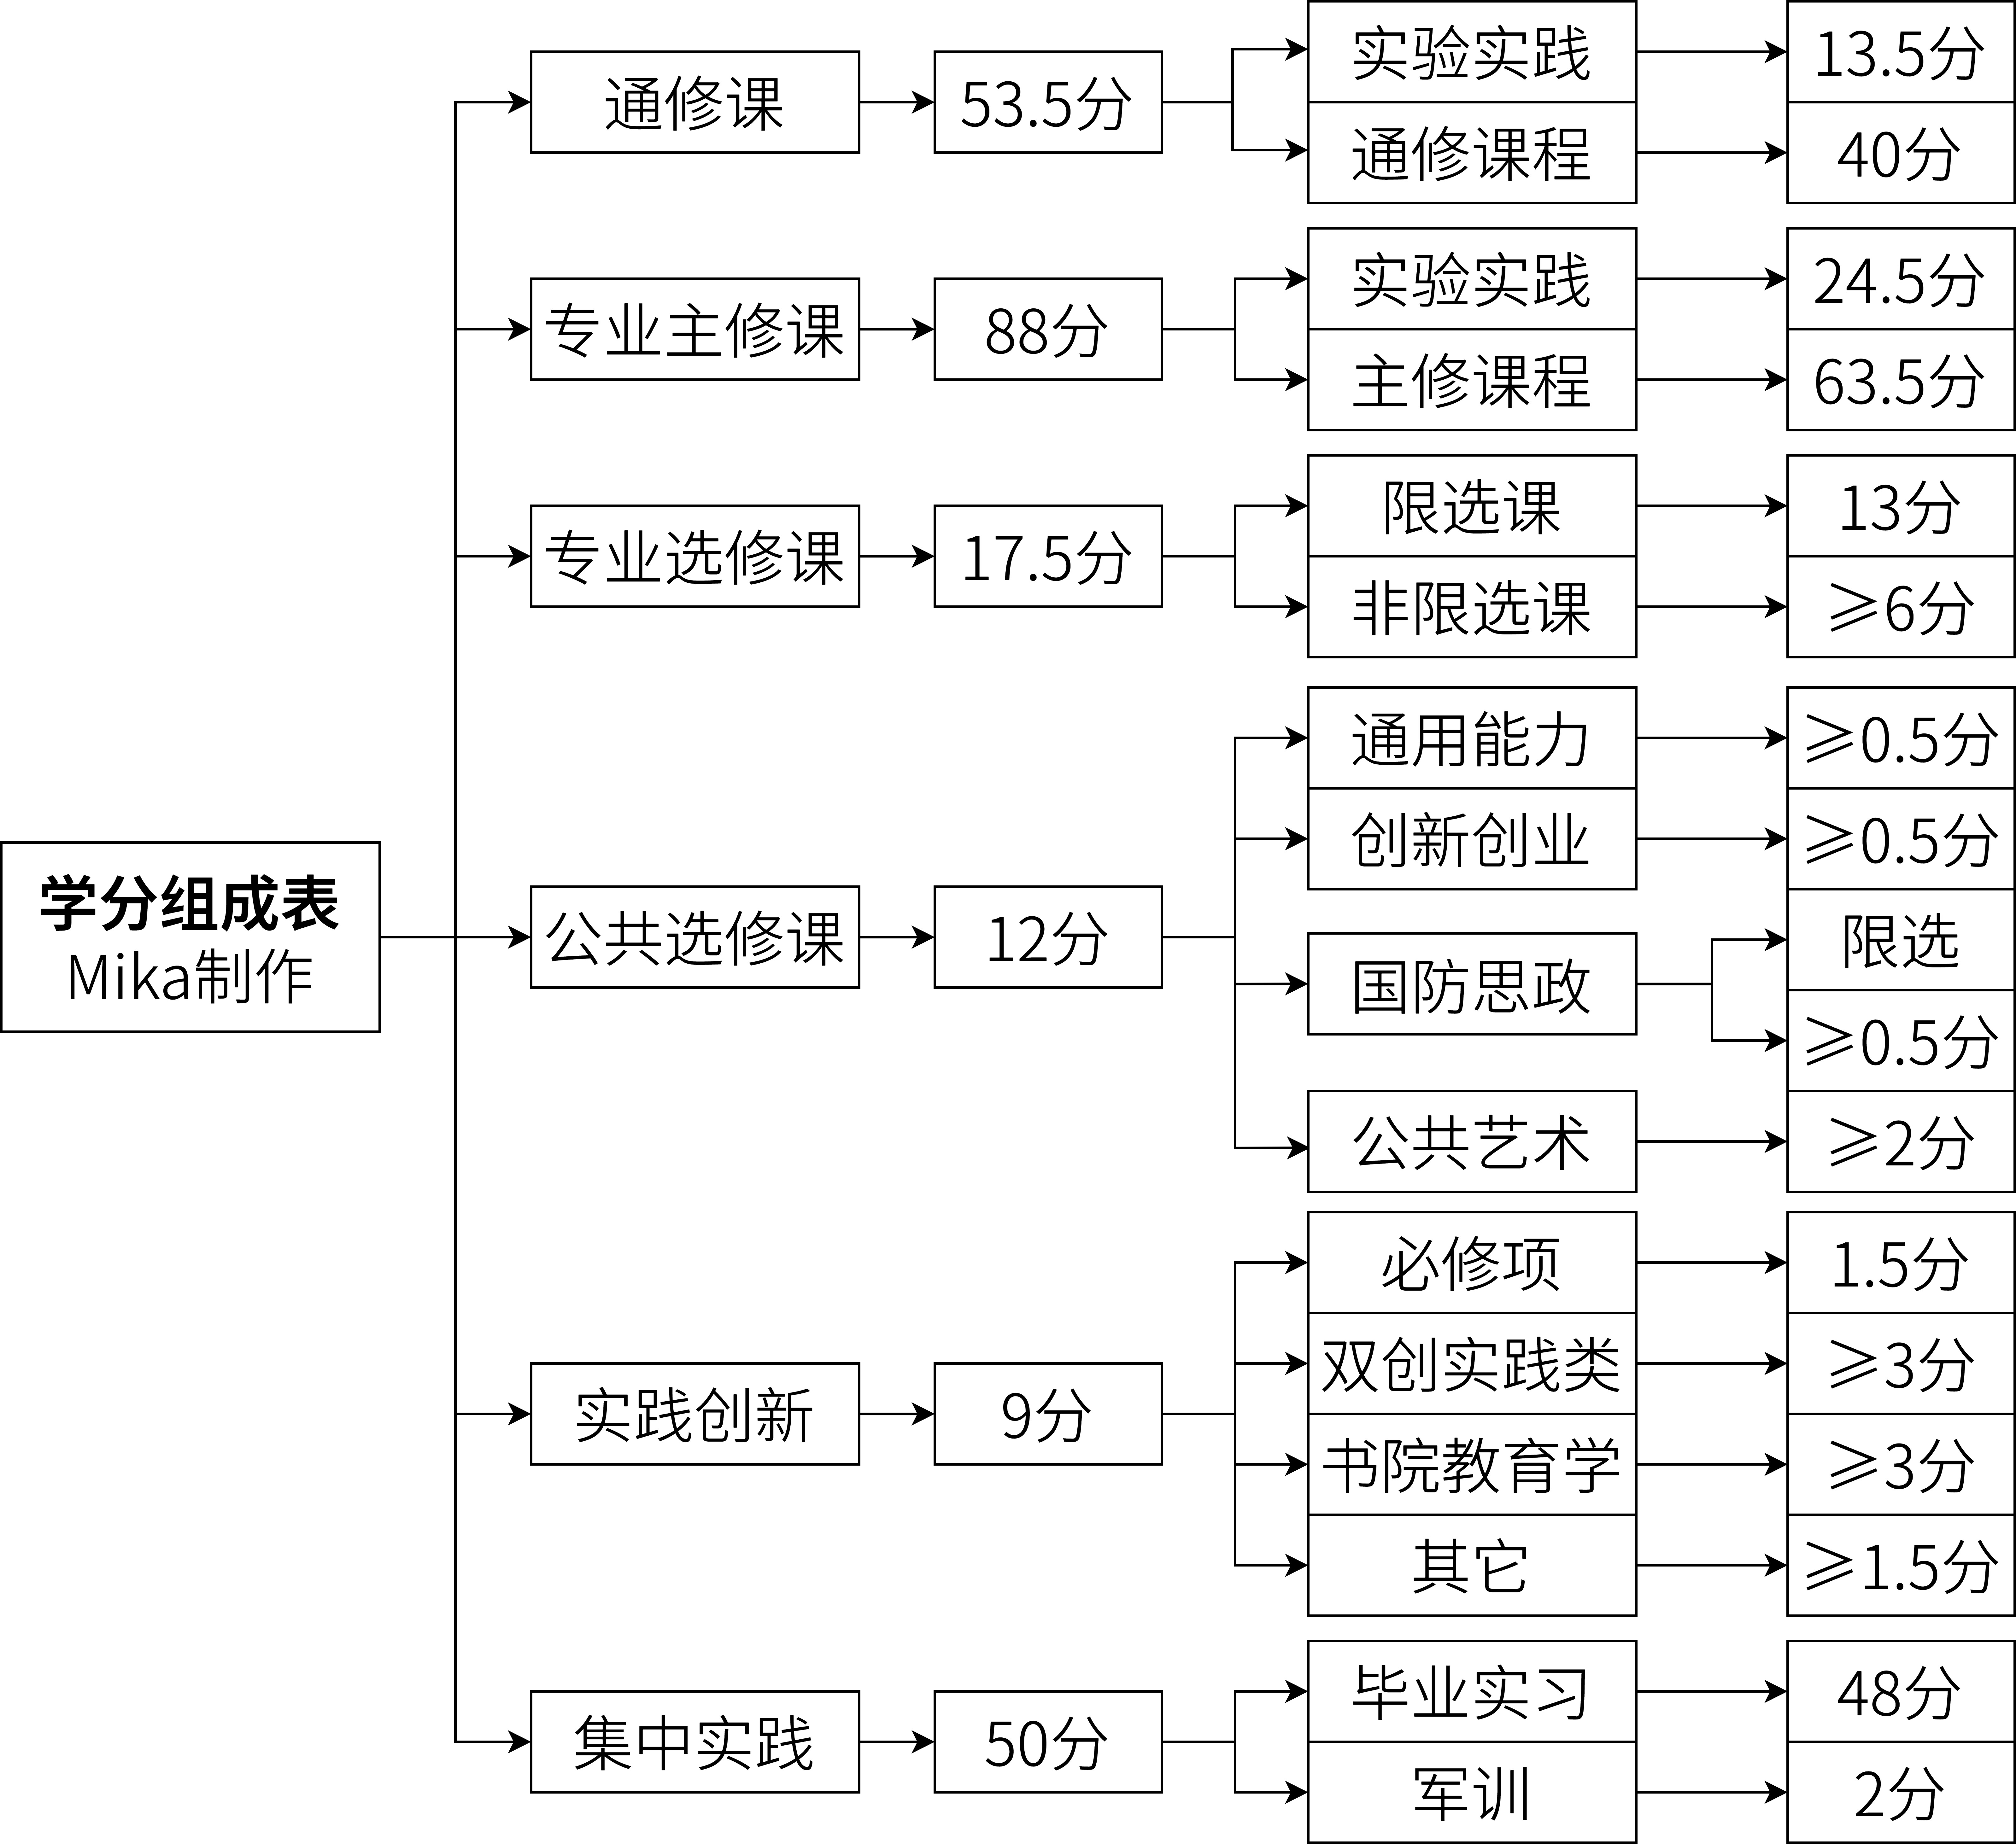
\includegraphics[width=\textwidth]{学分.jpg}
\end{table}

\section[学费]{学费}
\begin{enumerate}
    \item 学费收缴工作按照学校财务处通知进行,通常以班级为单位进行通知,可开具电子发票
    \item 如需申请助学贷款、生源地贷款等有特殊情况的同学可咨询学校财务处
    \item 选修课学费按照学分进行收费,所以同一个班的同学学费亦可不同,个人学费以\textbf{“潍坊医学院财务”公众号(潍坊医学院统一支付平台)}中的数据为准
    \item 选修课学分当前规定为1分/100元,多选课多交钱,少选课少交钱(希望大家如果看到了自己希望进一步学习的课程不要吝啬那几百块钱,选课机会只有一次,课程不会重开!)
    \item 此外,一定结合上面的说明修够学分,\textbf{修不够规定学分不能毕业}
\end{enumerate}